\documentclass[11pt,a4paper]{article}
\usepackage[T1]{fontenc}
\usepackage[utf8]{inputenc}
\usepackage[polish]{babel}
\usepackage[margin=2cm]{geometry}
\usepackage{graphicx}
\usepackage{amsmath}
\usepackage{booktabs}
\usepackage{listings}
\usepackage{xcolor}
\usepackage[hidelinks]{hyperref}

\lstset{
  language=C++,
  basicstyle=\ttfamily\scriptsize,
  breaklines=true,
  frame=single,
  tabsize=4,
  columns=fullflexible,
  keepspaces=true,
  numbers=left,
  numberstyle=\tiny\color{gray},
  backgroundcolor=\color{gray!8},
  extendedchars=true,
  literate={ą}{{\k{a}}}1 {ć}{{\'c}}1 {ę}{{\k{e}}}1 {ł}{{\l{}}}1 {ń}{{\'n}}1
           {ó}{{\'o}}1 {ś}{{\'s}}1 {ź}{{\'z}}1 {ż}{{\.z}}1 {Ł}{{\L{}}}1
           {Ź}{{\'Z}}1 {≈}{{$\approx$}}1
}
\newcommand{\kod}[3]{\lstinputlisting[firstline=#2,lastline=#3,firstnumber=#2]{kod/#1}}

\title{Usuwanie zanieczyszczeń falą uderzeniową -- symulacja w IGA-ADS}
\author{Rafał Szepieniec}
\date{\today}

\begin{document}
\maketitle

\section{Model}

Pole $u(x,y,t)$ to stężenie pary wodnej z cząstkami zanieczyszczeń na kwadracie
$[0,1]^2$ ($x$ poziomo, $y$ wysokość). Kod wyjściowy z zajęć (\texttt{heat\_2d.hpp},
\texttt{heat\_2d.cpp}) rozwiązuje jawną metodą Eulera równanie
\[
\frac{\partial u}{\partial t} = \Big(\frac{\partial T}{\partial y} + \mathrm{cannon}(x,y,t)\Big)\frac{\partial u}{\partial y}
+ K_x \frac{\partial^2 u}{\partial x^2} + K_y \frac{\partial^2 u}{\partial y^2} + f(y,t),
\]
gdzie:
\begin{itemize}
\item $K_x = 1$, $K_y = 0{,}1$ to dyfuzja;
\item $\partial T/\partial y = -5{,}2$ dla $y < 0{,}8$ i $0$ powyżej to gradient temperatury
  (inwersja na $y = 0{,}8$);
\item $f = (150 - 1200y)\,s(t)$ dla $y \le 0{,}125$ to emisja przy ziemi;
\item $\mathrm{cannon}$ to nasz dodatek.
\end{itemize}

Człon $c\,\partial u/\partial y$ z $c = \partial T/\partial y + \mathrm{cannon}$ to adwekcja
z prędkością $-c$ w kierunku $y$: dla $c < 0$ zanieczyszczenie wędruje w górę.
Dlatego $\partial T/\partial y = -5{,}2$ unosi chmurę z prędkością $5{,}2$, a powyżej inwersji
($c = 0$) unoszenie ustaje. Działko ma wartości \emph{ujemne}, więc dodaje prędkość w górę.

Dyskretyzacja (bez zmian względem kodu wyjściowego): $40\times40$ elementów, splajny stopnia 2,
$\Delta t = 10^{-5}$, 30\,000 kroków, czyli $t \in [0;\,0{,}3]$.
Jeden przebieg liczy się ok.\ 1,5\,min.

\section{Kod}

\subsection{Pliki i kompilacja}

Zmodyfikowane pliki \texttt{pollution.hpp} i \texttt{pollution.cpp} (pełny kod w dodatku~\ref{sec:kod})
leżą w \texttt{examples/pollution\_spcia/}. Do \texttt{examples/CMakeLists.txt} dodaliśmy wiersz:
\begin{lstlisting}[language=,numbers=none]
add_example(pollution_spcia GALOIS
  SRC
  pollution_spcia/pollution.cpp)
\end{lstlisting}
Program uruchamiamy poleceniem
\texttt{pollution\_spcia 40 2 8 [nazwa=wartość ...]}, np.\ \texttt{cannon\_t=0.16} lub
\texttt{cannon\_amp=0} (bez działka).

\subsection{Czas \texttt{t} w \texttt{compute\_rhs}}

Pętla czasu IGA-ADS (\texttt{simulation\_base.cpp}) w kroku numer $i$ liczy
$t = i\,\Delta t$ i wywołuje \texttt{before\_step(i, t)}, \texttt{step(i, t)}, \texttt{after\_step(i, t)}.
W kodzie wyjściowym \texttt{step} ignorował \texttt{t}, a \texttt{compute\_rhs()} nie miało argumentów.
Teraz \texttt{step} przekazuje \texttt{t} do \texttt{compute\_rhs}:
\kod{pollution.hpp}{88}{91}
Krok $i$ liczy więc $u^{i+1}$ z $u^{i}$, a działko jest brane w chwili $t = i \cdot 10^{-5}$
(jawny Euler bierze wszystkie człony z początku kroku). Krok $i$ odpowiada czasowi
$t = i\cdot 10^{-5}$, np.\ $t = 0{,}16$ to krok 16\,000.
Plik \texttt{out\_$i$.data} jest zapisywany po kroku $i$.

\subsection{Funkcja \texttt{cannon} i jej wywołanie}

\texttt{cannon(x, y, t)} jest liczona w każdym punkcie kwadratury:
$(x, y)$ = \texttt{point(e, q)}, czyli tak jak we wskazówce.
Wynik jest dodawany do \texttt{dTy(y)} w członie adwekcji:
\kod{pollution.hpp}{135}{159}

Działko i jego parametry:
\kod{pollution.hpp}{111}{133}
\kod{pollution.hpp}{24}{41}

\subsection{Pozostałe zmiany względem kodu wyjściowego}

\begin{itemize}
\item \textbf{Nazwy plików} \texttt{heat\_2d.*} $\to$ \texttt{pollution.*}, zgodnie z treścią
  zadania. Klasa nadal nazywa się \texttt{heat\_2d}.
\item \textbf{\texttt{compute\_rhs(iter, t)}}: \texttt{step} przekazuje czas \texttt{t},
  bo działko od niego zależy.
\item \textbf{\texttt{auto p = point(e, q)}} w \texttt{compute\_rhs}: współrzędne punktu kwadratury
  potrzebne do \texttt{cannon}.
\item \textbf{Wysokość w \texttt{f} i \texttt{dTy}} brana z punktu kwadratury zamiast
  \texttt{e2h(e[1])}. \texttt{e2h} dawało wysokość dolnej krawędzi elementu i działało tylko
  dla siatki z 40 elementami. Wysokość punktu jest dokładniejsza i nie zależy od siatki.
\item \textbf{Usunięte \texttt{y.fix\_right()}}, więc na górze jest $\nabla u\cdot n = 0$.
  Przy $u = 0$ na górze zanieczyszczenie, które doszło do $y = 1$, znikało z obszaru.
  Dół zostaje $u = 0$: unoszenie wnosi tędy powietrze, a od ziemi napływa czyste powietrze.
\item \textbf{Wydruk postępu} co 100 kroków w osobnych wierszach zamiast \texttt{\textbackslash r}
  w każdym kroku, żeby \texttt{log.txt} był czytelny.
\item \textbf{\texttt{main}}: siatka i parametry działka z linii poleceń oraz zapis
  \texttt{params.csv}. Kolejne przebiegi nie wymagają kompilacji, a każdy wynik jest opisany
  swoimi parametrami.
\item \textbf{Bez zmian}, aby porównanie z kodem wyjściowym było bezpośrednie: siatka
  $40\times40$, $p = 2$, $\Delta t = 10^{-5}$, 30\,000 kroków, zapis co 100 kroków na siatce
  $200\times200$, źródło, inwersja i dyfuzja.
\end{itemize}

\section{Wzór na działko}

\[
\mathrm{cannon}(x,y,t) = -A\;
\underbrace{\exp\!\Big(-\frac{(x - x_c)^2}{w^2}\Big)}_{\text{strumień}}\;
\underbrace{e^{-y/L}}_{\text{wysokość}}\;
\underbrace{\sin\!\Big(\pi\,\frac{t - t_k}{\tau}\Big)}_{\text{strzał}}
\quad\text{dla } t \in [t_k,\ t_k + \tau],\qquad t_k = t_0 + kP,\ k = 0, \dots, n_s - 1,
\]
a poza strzałami $0$. W kodzie jest to funkcja \texttt{cannon} (linie 116--133 w \texttt{pollution.hpp}).

\begin{center}
\begin{tabular}{@{}llrl@{}}
\toprule
Symbol & Znaczenie & Wartość & W kodzie \\
\midrule
$A$ & siła strzału & 80 & \texttt{cannon\_amp} \\
$x_c$ & położenie działka & 0,5 & \texttt{cannon\_x} \\
$w$ & szerokość strumienia & 0,08 & \texttt{cannon\_width} \\
$L$ & spadek z wysokością & 1,0 & \texttt{cannon\_reach} \\
$\tau$ & czas strzału & 0,03 (3000 kroków) & \texttt{cannon\_duration} \\
$P$ & odstęp strzałów & 0,06 (6000 kroków) & \texttt{cannon\_period} \\
$n_s$ & liczba strzałów & 2 & \texttt{cannon\_shots} \\
$t_0$ & początek strzelania & 0,005 / 0,07 / 0,16 & \texttt{cannon\_t} \\
\bottomrule
\end{tabular}
\end{center}

\paragraph{Czynniki wzoru.}
\begin{itemize}
\item \textbf{Strumień} $\exp(-(x - x_c)^2/w^2)$: działko stoi w jednym miejscu na ziemi
  i wymusza pionowy strumień powietrza nad sobą. Gauss daje strumień o szerokości ok.\ $2w = 0{,}16$
  (16\,\% obszaru), który łagodnie zanika na bokach. $w = 0{,}08$ to ok.\ 3 elementy siatki
  ($h = 0{,}025$), więc strumień jest dobrze rozwiązany numerycznie.
\item \textbf{Wysokość} $e^{-y/L}$: fala uderzeniowa słabnie, oddalając się od źródła.
  Przy $L = 1$ (wysokość obszaru) na inwersji zostaje $e^{-0{,}8} = 45\,\%$ siły, a na górze 37\,\%.
  Działko działa więc także ponad inwersją, gdzie $\partial T/\partial y = 0$, i tylko ono może
  przenieść tam zanieczyszczenie.
\item \textbf{Strzał} $\sin(\pi (t - t_k)/\tau)$ na $[t_k, t_k + \tau]$: pojedynczy wybuch narasta
  i wygasa łagodnie, bez skoku, który dawałby oscylacje. Strzały są powtarzane co $P$ z przerwą
  $P - \tau$: generator wybucha co ok.\ 10\,s, a w przerwie chmura może się ułożyć.
  Seria ma $n_s = 2$ strzały, potem działko milknie.
\end{itemize}

\paragraph{Wartości parametrów a wielkości modelu.}
\begin{itemize}
\item Bez działka chmura wznosi się z prędkością $5{,}2$, więc od ziemi do inwersji potrzebuje
  ok.\ $0{,}8 / 5{,}2 = 0{,}154$ (15\,400 kroków). Strzał $\tau = 0{,}03$ jest 5 razy krótszy,
  czyli jest impulsem, a nie stałym nadmuchem. Dwa strzały z przerwą zajmują $0{,}09$
  (9000 kroków, 30\,\% symulacji), więc mieszczą się w czasie symulacji dla każdego badanego $t_0$.
\item Siła $A = 80$ to 15-krotność prędkości wznoszenia $5{,}2$ przy ziemi i ok.\ 36 na inwersji.
  W jednym strzale strumień przesuwa się na wysokości inwersji o ok.\
  $36 \cdot \tfrac{2}{\pi} \cdot 0{,}03 \approx 0{,}7$. To wystarcza, aby przepchnąć chmurę przez
  warstwę $0{,}8$--$1$ w jednym strzale.
\item Stabilność: przesunięcie na krok $A\,\Delta t / h = 80 \cdot 10^{-5} / 0{,}025 = 0{,}032 \ll 1$,
  więc jawny schemat z $\Delta t = 10^{-5}$ zostaje stabilny.
\end{itemize}

\begin{figure}[htbp]
\centering
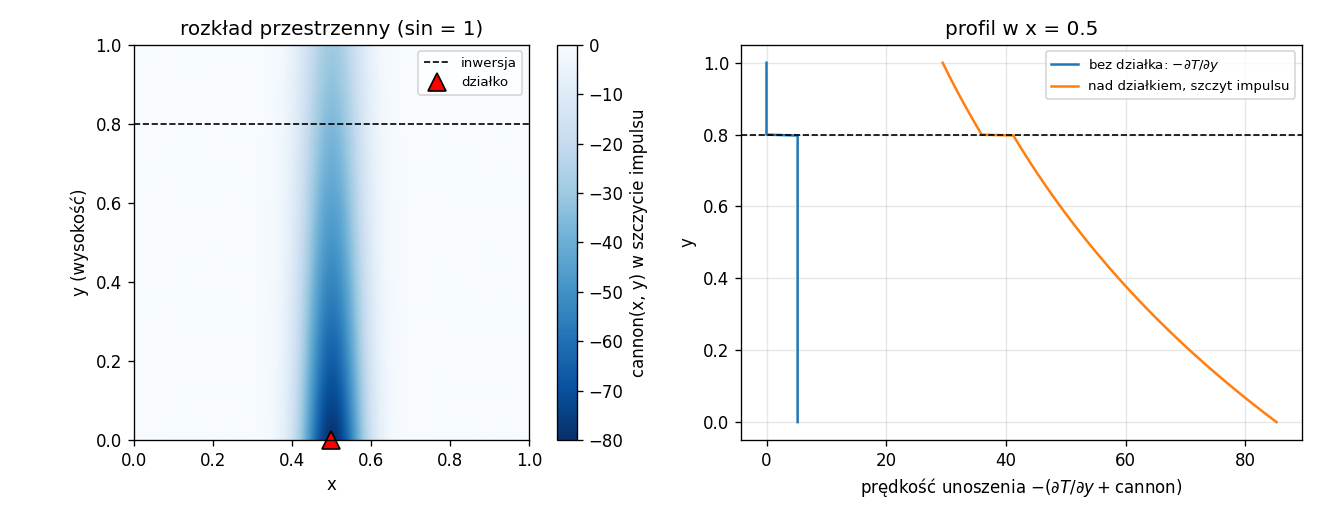
\includegraphics[width=\textwidth]{img/cannon_przestrzen.png}
\caption{Rozkład przestrzenny $\mathrm{cannon}(x,y)$ w szczycie strzału (lewy rysunek)
i prędkość unoszenia $-(\partial T/\partial y + \mathrm{cannon})$ nad działkiem (prawy rysunek):
bez działka $5{,}2$ pod inwersją i $0$ nad nią, w strzale ok.\ $85$ przy ziemi i $29$ na górze.}
\end{figure}

\begin{figure}[htbp]
\centering
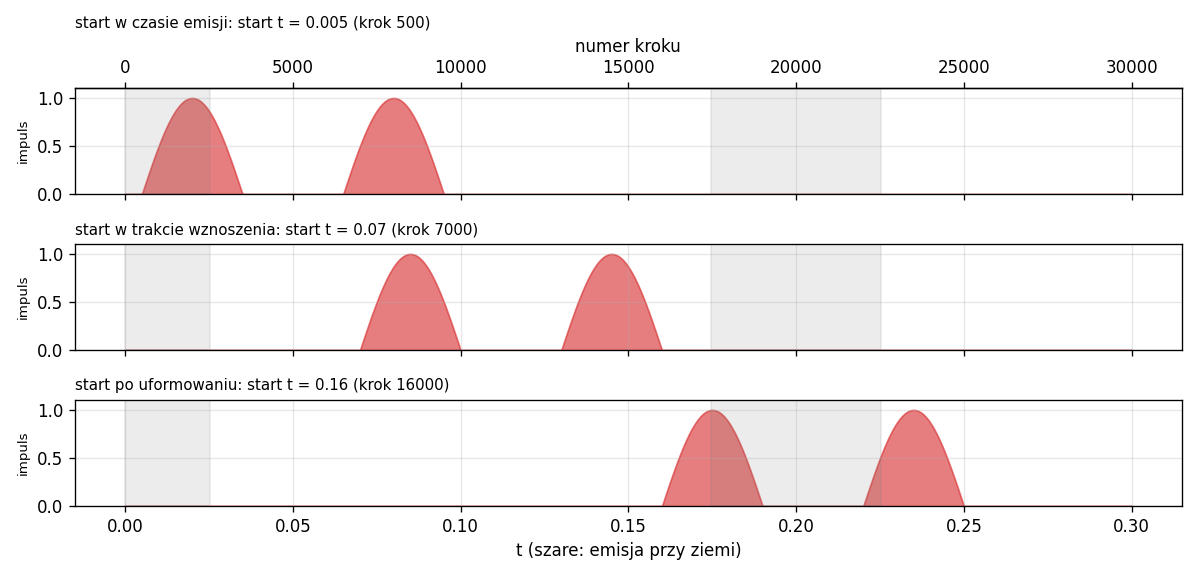
\includegraphics[width=\textwidth]{img/cannon_czas.png}
\caption{Zmienność działka w czasie dla trzech wariantów startu (oś dolna: czas modelu,
oś górna: numer kroku). Na szaro okresy emisji przy ziemi.}
\end{figure}

\section{Weryfikacja działania działka}

Symulacja kontrolna to działko w $x = 0{,}5$ ze startem po uformowaniu chmury: $t_0 = 0{,}16$.
Strzały trwają w krokach 16\,000--19\,000 ($t = 0{,}16$--$0{,}19$) i 22\,000--25\,000
($t = 0{,}22$--$0{,}25$). Strzelanie kończy się w kroku 25\,000 ($t = 0{,}25$).
Porównujemy ją z symulacją bez działka (\texttt{cannon\_amp=0}, poza tym ten sam kod).

\begin{figure}[htbp]
\centering
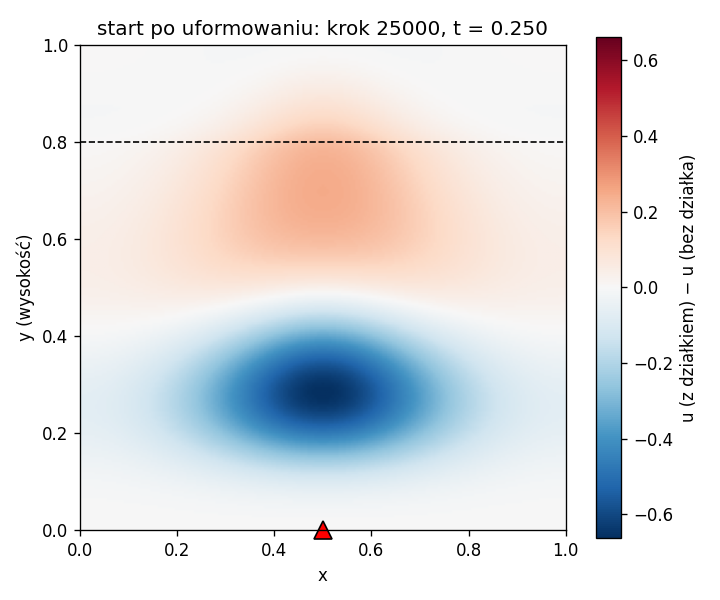
\includegraphics[width=0.55\textwidth]{img/roznica.png}
\caption{Różnica stężeń (z działkiem minus bez działka) w kroku 25\,000, na końcu strzelania.}
\end{figure}

Działko przenosi zanieczyszczenia \textbf{w górę, nad sobą}. Spod $y \approx 0{,}3$ w pasie
$x \approx 0{,}3$--$0{,}7$ ubyło (na niebiesko), a przybyło wyżej, głównie tuż pod
inwersją ($y \approx 0{,}5$--$0{,}8$) i nieco nad nią (na czerwono). Daleko od działka ($x < 0{,}2$, $x > 0{,}8$) różnica jest bliska zeru.

\section{Animacje}

Animacje są w osobnych plikach w katalogu \texttt{anim/}:
\begin{itemize}
\item \texttt{bez\_dzialka.gif}: kod wyjściowy, bez działka,
\item \texttt{start\_emisja.gif}: start $t_0 = 0{,}005$,
\item \texttt{start\_wznoszenie.gif}: start $t_0 = 0{,}07$,
\item \texttt{start\_po\_uformowaniu.gif}: start $t_0 = 0{,}16$.
\end{itemize}
Wszystkie klatki wszystkich animacji mają tę samą skalę barw ($u \in [0, 1]$). Każda klatka ma:
\begin{itemize}
\item opisane osie i legendę skali,
\item numer kroku i czas w tytule; w czasie strzału tytuł jest czerwony z napisem ,,STRZAŁ'',
\item linię inwersji $y = 0{,}8$ i położenie działka (czerwony trójkąt).
\end{itemize}

\section{Klatki z wybranych kroków}

Wszystkie klatki pochodzą z symulacji kontrolnej ($t_0 = 0{,}16$) i mają tę samą skalę barw co animacje.

\begin{figure}[htbp]
\centering
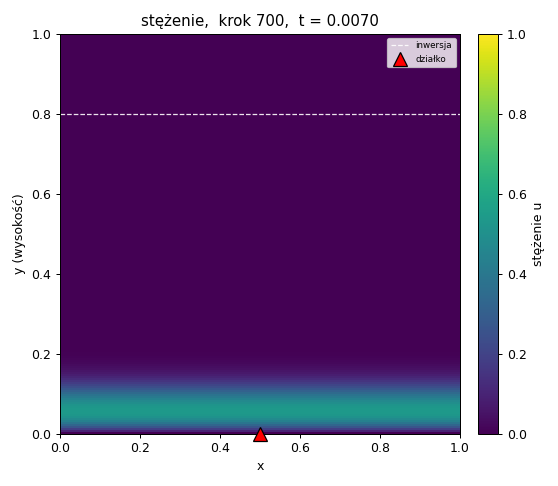
\includegraphics[width=0.32\textwidth]{img/k_00700.png}\hfill
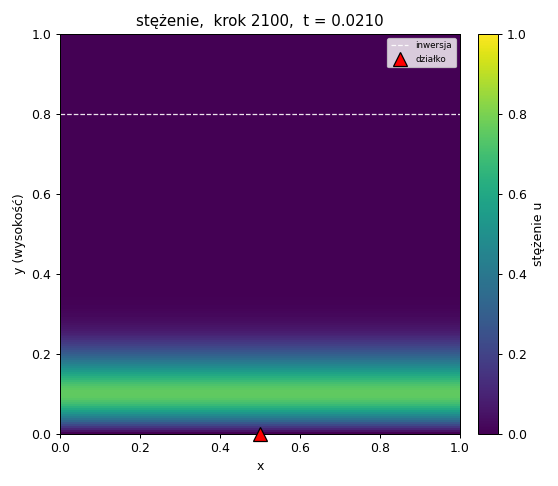
\includegraphics[width=0.32\textwidth]{img/k_02100.png}\hfill
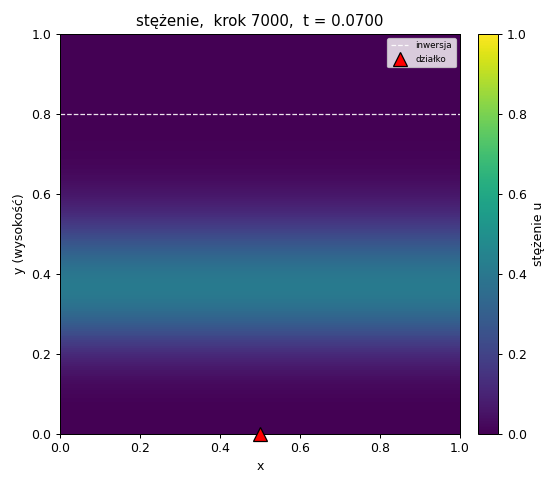
\includegraphics[width=0.32\textwidth]{img/k_07000.png}
\caption{\textbf{Krok 700} ($t = 0{,}007$), emisja przy ziemi: $s(t)$ jest bliskie 1, źródło
$f$ działa w $y \le 0{,}125$. \textbf{Krok 2100} ($t = 0{,}021$), koniec emisji: $s(t)$ maleje
do 0 w kroku 2531, a warstwa już się unosi. \textbf{Krok 7000} ($t = 0{,}07$), wznoszenie:
chmura jako pas przesuwa się w górę z prędkością $5{,}2$ (człon $\partial T/\partial y\,\partial u/\partial y$)
i rozmywa się przez dyfuzję.}
\end{figure}

\begin{figure}[htbp]
\centering
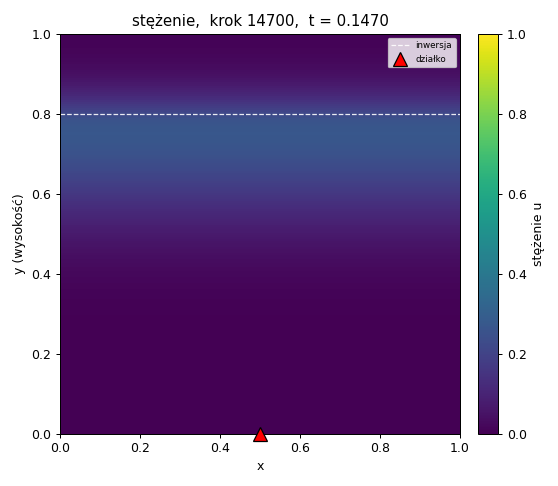
\includegraphics[width=0.32\textwidth]{img/k_14700.png}\hfill
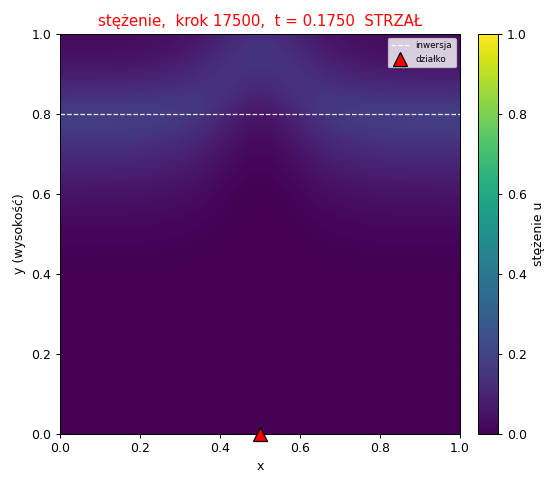
\includegraphics[width=0.32\textwidth]{img/k_17500.png}\hfill
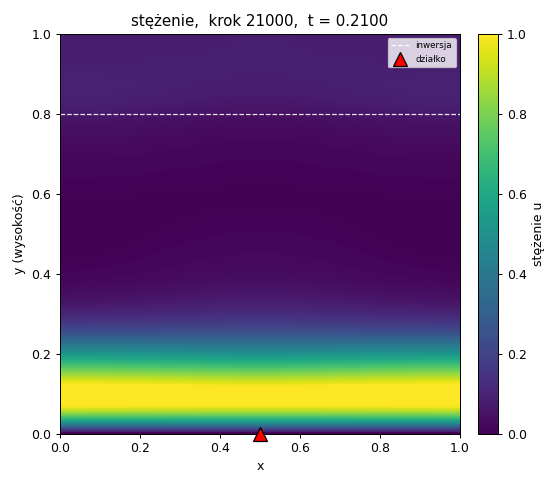
\includegraphics[width=0.32\textwidth]{img/k_21000.png}
\caption{\textbf{Krok 14\,700} ($t = 0{,}147$), chmura pod inwersją: nad $y = 0{,}8$ prędkość
unoszenia jest zerowa, więc chmura zatrzymuje się i zagęszcza pod inwersją.
\textbf{Krok 17\,500} ($t = 0{,}175$), szczyt pierwszego strzału: nad działkiem prędkość unoszenia
rośnie do ok.\ 36 na inwersji i resztka chmury przechodzi ponad $y = 0{,}8$.
\textbf{Krok 21\,000} ($t = 0{,}21$), druga emisja ($s(t) > 0$ od kroku 17\,469) w przerwie
między strzałami: nowy pas przy ziemi.}
\end{figure}

\begin{figure}[htbp]
\centering
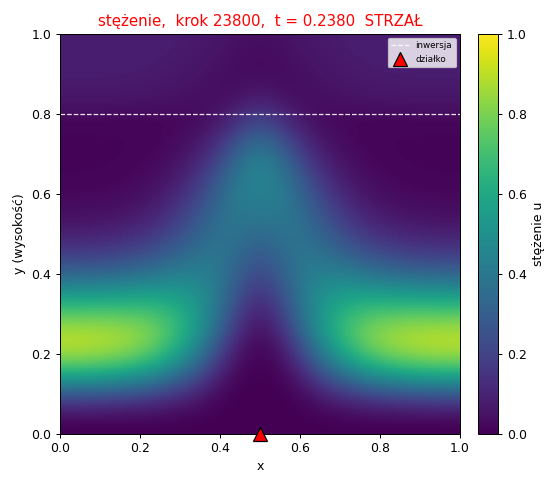
\includegraphics[width=0.32\textwidth]{img/k_23800.png}\hfill
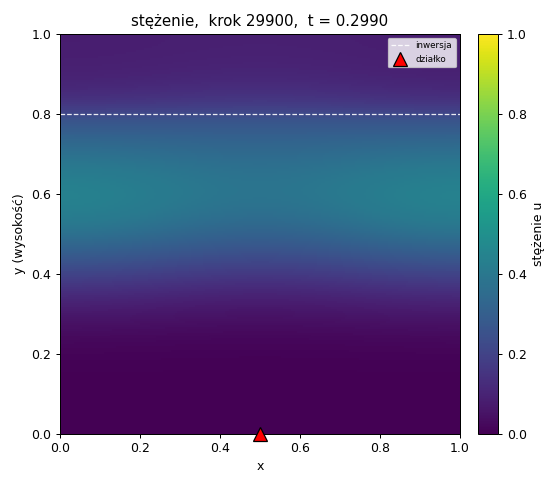
\includegraphics[width=0.32\textwidth]{img/k_29900.png}
\caption{\textbf{Krok 23\,800} ($t = 0{,}238$), szczyt drugiego strzału: strumień wygina pas
w górę nad działkiem. \textbf{Krok 29\,900} ($t = 0{,}299$), koniec: nad działkiem jest
,,komin'', którym zanieczyszczenie przeszło przez inwersję. Pod nim jest czysto, a po bokach
chmura stoi pod inwersją.}
\end{figure}

\begin{figure}[htbp]
\centering
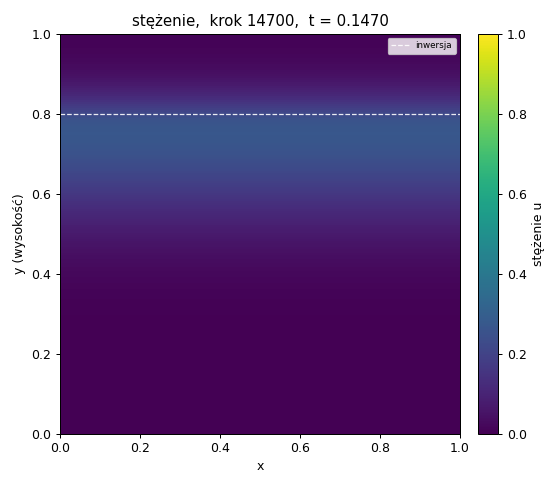
\includegraphics[width=0.24\textwidth]{img/b_14700.png}\hfill
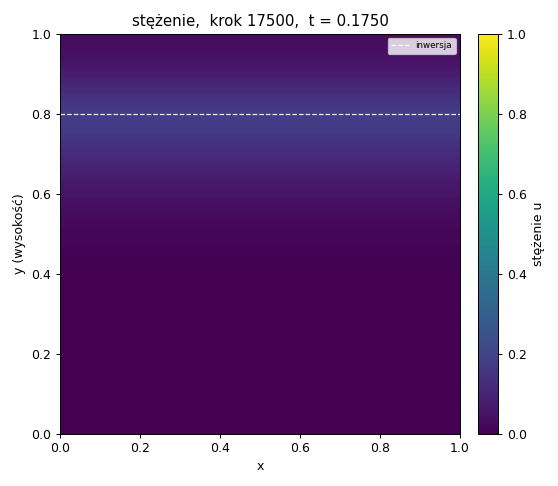
\includegraphics[width=0.24\textwidth]{img/b_17500.png}\hfill
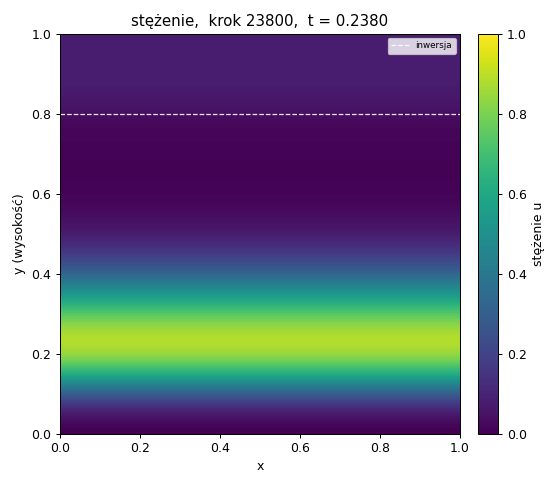
\includegraphics[width=0.24\textwidth]{img/b_23800.png}\hfill
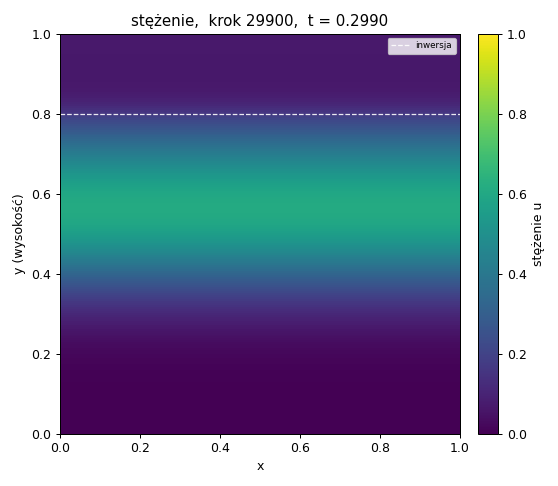
\includegraphics[width=0.24\textwidth]{img/b_29900.png}
\caption{Te same kroki (14\,700, 17\,500, 23\,800, 29\,900) bez działka: pas wznosi się
równomiernie w całej szerokości i staje pod inwersją.}
\end{figure}

\section{Czy ze strzelaniem należy poczekać, aż chmura się uformuje?}

\subsection{Powstawanie chmury (symulacja bez działka)}

\begin{itemize}
\item \textbf{Emisja.} Źródło \texttt{f} (linie 99--103) jest mnożone przez
  $s = \max\big((\cos(\pi i / 10^4) - 0{,}7)/0{,}3,\ 0\big)$ z \texttt{before\_step} (linia 83).
  $s > 0$ dla kroków 0--2531 ($t < 0{,}0253$) i ponownie 17\,469--22\,531
  ($t = 0{,}175$--$0{,}225$). Druga emisja tworzy drugą chmurę.
\item \textbf{Wznoszenie.} Środek masy chmury rośnie liniowo z prędkością $5{,}17$
  (dopasowanie dla $t = 0{,}03$--$0{,}10$, rys.~\ref{fig:wzn}). W kodzie jest $5{,}2$.
\item \textbf{Dojście do inwersji.} Górna krawędź chmury (połowa maksimum) dochodzi do
  $y = 0{,}8$ w kroku 11\,600 ($t = 0{,}116$).
\item \textbf{Uformowanie.} Chmurę uznajemy za uformowaną, gdy środek masy zwalnia poniżej
  połowy prędkości wznoszenia, czyli chmura hamuje pod inwersją: od kroku 14\,800
  ($t = 0{,}148$). Oderwanie od ziemi następuje tuż po końcu emisji (krok 2531).
\end{itemize}

\begin{figure}[htbp]
\centering
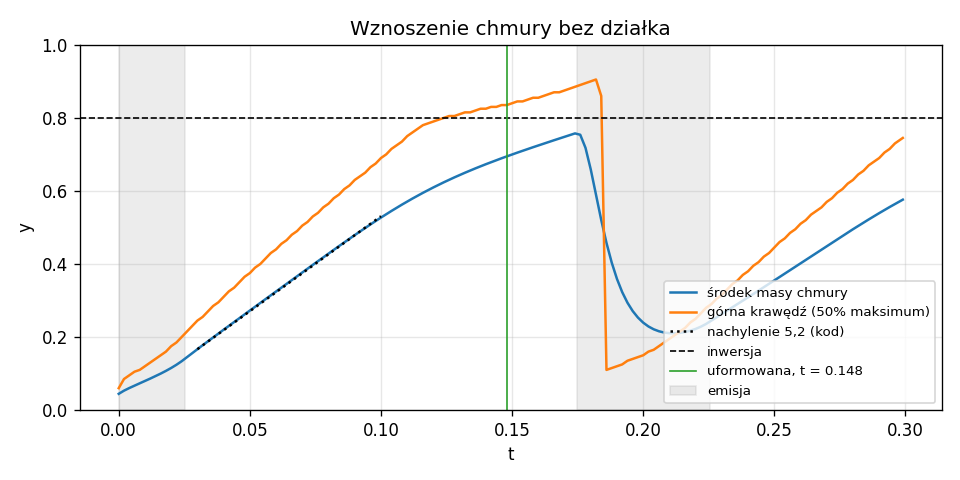
\includegraphics[width=0.75\textwidth]{img/wznoszenie.png}
\caption{Wysokość chmury w czasie bez działka.}
\label{fig:wzn}
\end{figure}

\subsection{Eksperyment}

Cztery symulacje różnią się wyłącznie krokiem pierwszego strzału. Wszystkie mają to samo działko
i ten sam harmonogram: 2 strzały po 3000 kroków co 6000 kroków.

\begin{center}
\begin{tabular}{@{}llll@{}}
\toprule
Wariant & Start & Strzały (kroki) & Stan chmury przy starcie \\
\midrule
bez działka & -- & -- & odniesienie \\
w czasie emisji & $t_0 = 0{,}005$ & 500--3500, 6500--9500 & przy ziemi, przed oderwaniem \\
w trakcie wznoszenia & $t_0 = 0{,}07$ & 7000--10\,000, 13\,000--16\,000 & w połowie drogi do inwersji \\
po uformowaniu & $t_0 = 0{,}16$ & 16\,000--19\,000, 22\,000--25\,000 & pod inwersją \\
\bottomrule
\end{tabular}
\end{center}

\subsection{Cele i miary}

\begin{itemize}
\item \textbf{Cel 1: ochrona ludzi przy ziemi.} Miara: średnie w czasie stężenie w warstwie
  $y < 0{,}1$, czyli $\frac{1}{0{,}3}\int_0^{0{,}3} \bar u_{y<0{,}1}\,dt$.
\item \textbf{Cel 2: usunięcie zanieczyszczeń spod inwersji.} Miara: ilość pod inwersją
  $\int_{y<0{,}8} u$, średnio w czasie oraz na końcu ($t = 0{,}3$).
\end{itemize}

\begin{figure}[htbp]
\centering
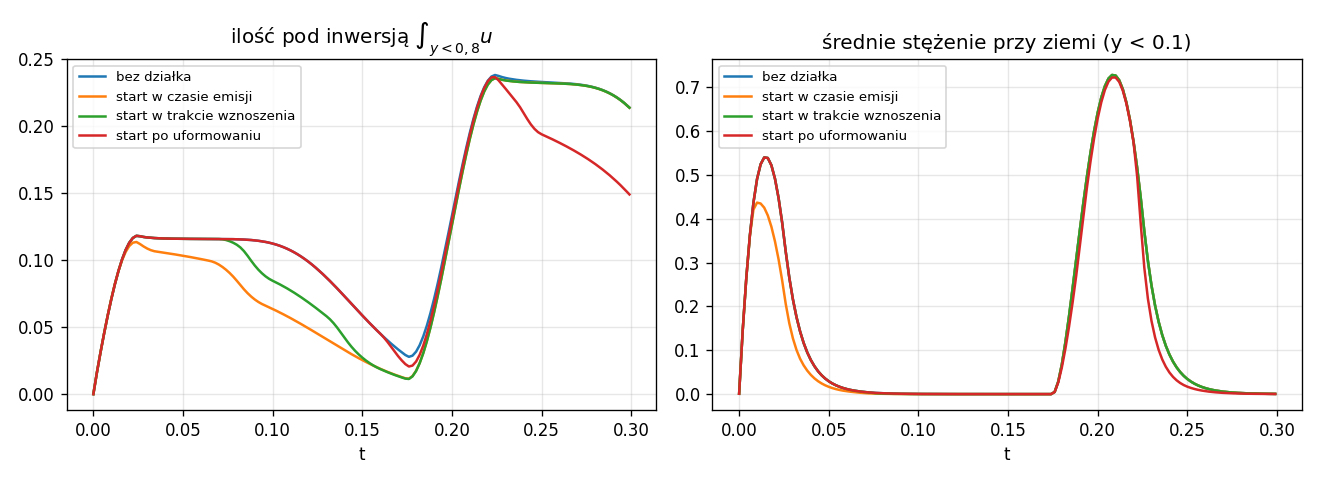
\includegraphics[width=\textwidth]{img/miary.png}
\caption{Ilość pod inwersją i średnie stężenie przy ziemi w czasie.}
\end{figure}

\begin{table}[htbp]
\centering
\begin{tabular}{@{}lcccc@{}}
\toprule
& \multicolumn{1}{c}{Cel 1} & \multicolumn{3}{c}{Cel 2: ilość pod inwersją} \\
\cmidrule(lr){2-2}\cmidrule(lr){3-5}
Wariant & przy ziemi, średnio & w $t = 0{,}17$ & średnio & na końcu \\
\midrule
bez działka & 0,139 & 0,033 & 0,134 & 0,214 \\
w czasie emisji & \textbf{0,128} ($-8\,\%$) & 0,014 & \textbf{0,117} ($-13\,\%$) & 0,214 \\
w trakcie wznoszenia & 0,139 & \textbf{0,013} & 0,124 ($-7\,\%$) & 0,214 \\
po uformowaniu & 0,132 ($-5\,\%$) & 0,028 & 0,122 ($-9\,\%$) & \textbf{0,149} ($-30\,\%$) \\
\bottomrule
\end{tabular}
\caption{Miary dla wszystkich symulacji. W $t = 0{,}17$ żaden wariant nie zaczął jeszcze
działać na drugą chmurę, więc ta kolumna dotyczy tylko pierwszej chmury.}
\end{table}

\subsection{Odpowiedź}

Odpowiedź jest \textbf{warunkowa}: zależy od celu.
\begin{itemize}
\item \textbf{Cel 1 (ludzie przy ziemi): nie czekać.} Najlepiej strzelać w czasie emisji.
  Tylko wtedy zanieczyszczenie jest przy ziemi, a działko ma przy ziemi największą siłę
  ($A e^{0} = 80$ wobec $5{,}2$). Chmura szybciej odrywa się od ziemi i szczyt stężenia przy
  ziemi spada z 0,54 do 0,43. Później przy ziemi nic nie ma (do drugiej emisji), więc strzały
  nic tam nie zmieniają.
\item \textbf{Cel 2 dla pierwszej chmury: też nie czekać.} Pod inwersją działko tylko dodaje
  prędkość do $5{,}2$, które i tak unosi chmurę, więc przyspiesza jej dojście do $y = 0{,}8$.
  Na inwersji chmura traci masę (punkt~\ref{sec:masa}). W $t = 0{,}17$ pod inwersją zostaje
  0,013--0,014 przy wczesnym starcie, a 0,028 przy starcie po uformowaniu.
\item \textbf{Stan końcowy: czekać.} Wartość na końcu zmienia tylko start po uformowaniu
  ($-30\,\%$), bo jego strzały (do kroku 25\,000) trafiają w drugą chmurę.
  Wcześniejsze strzały kończą się przed drugą emisją, więc na końcu nie ma po nich śladu.
\end{itemize}

Wynika to z równania. Działko zmienia tylko prędkość unoszenia $-c$. Pod inwersją $c$ jest już
ujemne, więc strzał przyspiesza ruch, który i tak by nastąpił. Ponad inwersją $c = 0$ i tylko
strzał przenosi tam zanieczyszczenie, ale jest tam ono dopiero wtedy, gdy chmura doszła do
$y = 0{,}8$. Działko pomaga więc tam, gdzie w danej chwili jest zanieczyszczenie: przy ziemi
w czasie emisji, a pod inwersją po jej uformowaniu.

\section{Czy działko usuwa zanieczyszczenia?}
\label{sec:masa}

\begin{figure}[htbp]
\centering
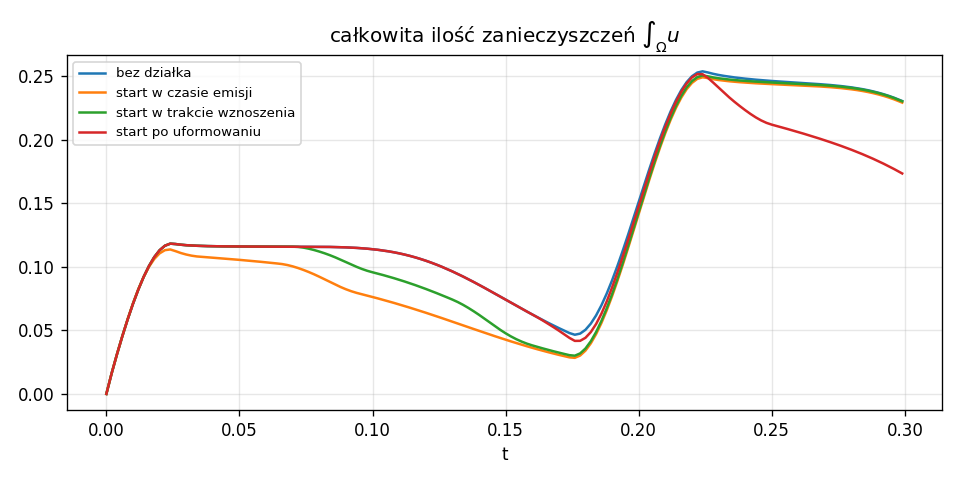
\includegraphics[width=0.48\textwidth]{img/masa_calkowita.png}\hfill
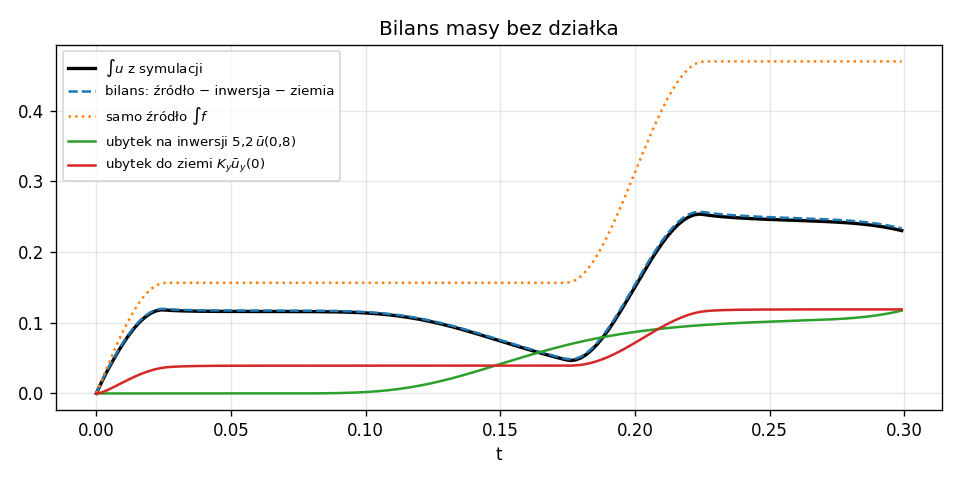
\includegraphics[width=0.48\textwidth]{img/bilans.png}
\caption{Całkowita ilość zanieczyszczeń $\int_\Omega u$ w czasie (lewy rysunek) i jej bilans
z członów równania bez działka (prawy rysunek).}
\end{figure}

Całkując równanie po obszarze (z $u = 0$ na dole, $\nabla u\cdot n = 0$ na górze i bokach):
\[
\frac{d}{dt}\int_\Omega u
= \underbrace{\int_\Omega f}_{\text{emisja}}
\;-\; \underbrace{K_y\!\int_0^1 \frac{\partial u}{\partial y}\Big|_{y=0} dx}_{\text{osiadanie na ziemi}}
\;-\; \underbrace{\int_\Omega \frac{\partial c}{\partial y}\,u}_{\text{zmiana prędkości}}
\;+\; \underbrace{\int_0^1 c\,u\,\Big|_{y=1} dx}_{\text{wypływ górą}} .
\]

\begin{itemize}
\item \textbf{Emisja} $\int f = 9{,}375\,s(t)$ (linie 100--103) dodaje razem 0,470.
\item \textbf{Osiadanie na ziemi.} Warunek $u = 0$ na dole (linia 63) daje dyfuzyjny wypływ
  do ziemi: 0,119.
\item \textbf{Ubytek na inwersji.} Na $y = 0{,}8$ prędkość $c$ skacze z $-5{,}2$ do 0, więc
  $\partial c/\partial y = 5{,}2\,\delta(y - 0{,}8)$, co daje ubytek
  $5{,}2\int u(x, 0{,}8)\,dx$: razem 0,117.
\end{itemize}

Bez działka bilans daje na końcu 0,234, a symulacja 0,230. Każda zmiana całkowitej ilości
wynika więc z tych trzech członów.

Ubytek na inwersji wynika z postaci równania z zajęć: adwekcja
$c\,\partial u/\partial y$ nie zachowuje masy tam, gdzie prędkość się zmienia. W postaci
$\partial(cu)/\partial y$ chmura gromadziłaby się pod inwersją bez strat.

\paragraph{Z działkiem} (start po uformowaniu) dochodzą dwa człony:
\begin{itemize}
\item w kolumnie działka $\partial c/\partial y = (A/L)\,e^{-y/L}\cdots > 0$, czyli ubytek
  proporcjonalny do $u$ w strumieniu;
\item na górze $c = \mathrm{cannon} < 0$, czyli wypływ $c\,u$ przez $y = 1$ w czasie strzału.
\end{itemize}
Na końcu całkowita ilość spada z 0,230 do 0,173 (o 0,057), a nad inwersją rośnie tylko
z 0,016 do 0,024 (o 0,008).

Działko więc \textbf{przemieszcza} zanieczyszczenia w górę, nad siebie (rys.\ różnicy), ale
w tym modelu większość ubytku spod inwersji ($0{,}065$) to nie przeniesienie, tylko ubytek
z członów $\partial c/\partial y$ i wypływ górą. Fizycznie odpowiada to wyrzuceniu
zanieczyszczeń ponad obszar modelu, a nie ich zniszczeniu.

\begin{thebibliography}{9}
\bibitem{misan} K. Misan i in., \emph{Fast isogeometric analysis simulations of a process of air
  pollution removal by artificially generated shock waves}, LNCS 13352 (ICCS 2022) 298--311.
\bibitem{ads} M. Łoś i in., \emph{IGA-ADS: Isogeometric analysis FEM using ADS solver},
  Computer Physics Communications 217 (2017) 99--116.
\end{thebibliography}

\appendix
\section{Kod}
\label{sec:kod}

Kod wyjściowy z zajęć jest dla porównania w \texttt{kod/oryginal/}.

\subsection*{pollution.hpp}
\lstinputlisting{kod/pollution.hpp}

\subsection*{pollution.cpp}
\lstinputlisting{kod/pollution.cpp}

\end{document}
